\documentclass{beamer}
\usepackage[utf8]{inputenc}
\usepackage[T1]{fontenc}
\usepackage{mathabx}
\usepackage{mathpazo}
\usepackage{eulervm}
\usepackage{natbib}
\usepackage{multimedia}


%% Load the markdown package
\usepackage[citations,footnotes,definitionLists,hashEnumerators,smartEllipses,tightLists=false,pipeTables,tableCaptions,hybrid]{markdown}
%%begin novalidate
\markdownSetup{rendererPrototypes={
 link = {\href{#2}{#1}},
 headingOne = {\section{#1}},
 headingTwo = {\subsection{#1}},
 headingThree = {\begin{frame}\frametitle{#1}},
 headingFour = {\begin{block}{#1}},
 horizontalRule = {\end{block}}
}}
%%end novalidate

\usetheme{Boadilla}
\usefonttheme{serif}
\usecolortheme{beaver}


\title{WaveNet - Generative Music Production}
\author{Simon Scapan}
\institute{DHBW - Mannheim}

\begin{document}

\maketitle

\frame{\tableofcontents}

\begin{markdown}
%%begin novalidate

%%%%%%%%%%%%%%%%%%%%%%%%%%%%%%%%%%%%%%%%%%%%%%%%%%%%%%%%%%%%%%%%%%%%%%%

# WaveNet in General

### WaveNet in General

-  Developed by DeepMind in London
- Generate raw speech signals with subjective naturalness never before reported in the field of Text-to-Speech ( TTS ) 
\linebreak
[@paper_oord_dieleman_2016]
- Performance improvement by over 50\% 
\linebreak
[@webpage_oord_dieleman_2016]
- Advantage : one model for different purposes

\end{frame}
%%%%%%%%%%%%%%%%%%%%%%%%%%%%%%%%%%%%%%%%%%%%%%%%%%%%%%%%%%%%%%%%%%%%%%%

### WaveNet in General

- Architecture based on dilated causal convolutions
- WaveNets provide a generic and flexible framework for many applications relying on audio generation :
    * Text-to-Speech
    * Music generation
    * Speech enhancement
    * Voice conversion
    * Source separation
    
\vspace{1cm}
Source : [@paper_oord_dieleman_2016]
\end{frame}
%%%%%%%%%%%%%%%%%%%%%%%%%%%%%%%%%%%%%%%%%%%%%%%%%%%%%%%%%%%%%%%%%%%%%%%

# Model Explanation

## Theoreticaly

### Model Explanation - Theoreticaly

- Generative model operating on raw audio waveform
- Joint probability of a waveform is factorised as product of conditional probabilities
- Each audio sample is therefore conditioned on the samples at all previous timesteps
- Conditional probability distribution is modelled by stack of convolutional layers
- No pooling layers in network
- Output of the model has same time dimensionality as input

\vspace{1cm}
Source : [@paper_oord_dieleman_2016]
\end{frame}
%%%%%%%%%%%%%%%%%%%%%%%%%%%%%%%%%%%%%%%%%%%%%%%%%%%%%%%%%%%%%%%%%%%%%%%

### Model Explanation - Visual

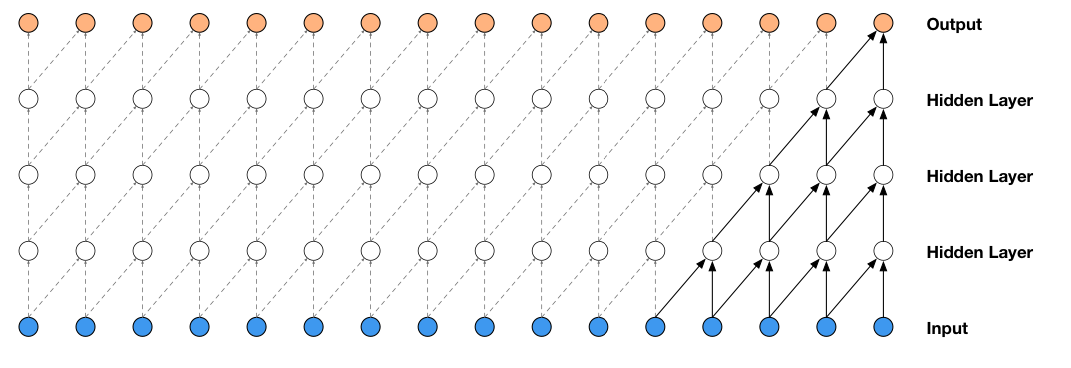
\includegraphics[scale=0.3]{CausalConvolutions.png}
Figure : Visualization of a stack of causal convolutional layers 
\linebreak
Source : [@paper_oord_dieleman_2016]

\end{frame}
%%%%%%%%%%%%%%%%%%%%%%%%%%%%%%%%%%%%%%%%%%%%%%%%%%%%%%%%%%%%%%%%%%%%%%%

## Causal Convolutions

### Model Explanation - Causal Convolutions

- Main ingredient of WaveNet are causal convolutions
- Based on that, the model cannot violate the ordering in which the data is modeled
- Predictions emitted by model at timestep t cannot depend on any of the future timesteps
- At training, conditional predictions for all timesteps can be made in parallel ( all timesteps of ground truth x are known )

\vspace{1cm}
Source : [@paper_oord_dieleman_2016]
\end{frame}
%%%%%%%%%%%%%%%%%%%%%%%%%%%%%%%%%%%%%%%%%%%%%%%%%%%%%%%%%%%%%%%%%%%%%%%

### Model Explanation - Causal Convolutions

- At generation of outputs with model, predictions are sequential : \linebreak
    after each sample is predicted, it is fed back into network to predict next sample
- Models with causal convolutions do not have recurrent connections, they are typically faster to train than RNNs
- Problem of causal convolutions is : they require many layers, or large filters to increase the receptive field

\vspace{1cm}
Source : [@paper_oord_dieleman_2016]
\end{frame}
%%%%%%%%%%%%%%%%%%%%%%%%%%%%%%%%%%%%%%%%%%%%%%%%%%%%%%%%%%%%%%%%%%%%%%%

## Dilated Convolutions

### Model Explanation - Dilated Convolutions

- A dilated convolution is a convolution where the filter is applied over an area larger than its length by skipping input values with a certain step
- It is equivalent to a convolution with a larger filter derived from the original filter by dilating it with zeros, but significantly more efficient
- Similar to pooling or strided convolutions, but here the output has the same size as the input
- Stacked dilated convolutions enable networks to have very large receptive fields with just a few layers

\vspace{1cm}
Source : [@paper_oord_dieleman_2016]
\end{frame}
%%%%%%%%%%%%%%%%%%%%%%%%%%%%%%%%%%%%%%%%%%%%%%%%%%%%%%%%%%%%%%%%%%%%%%%

### Model Explanation - Visual

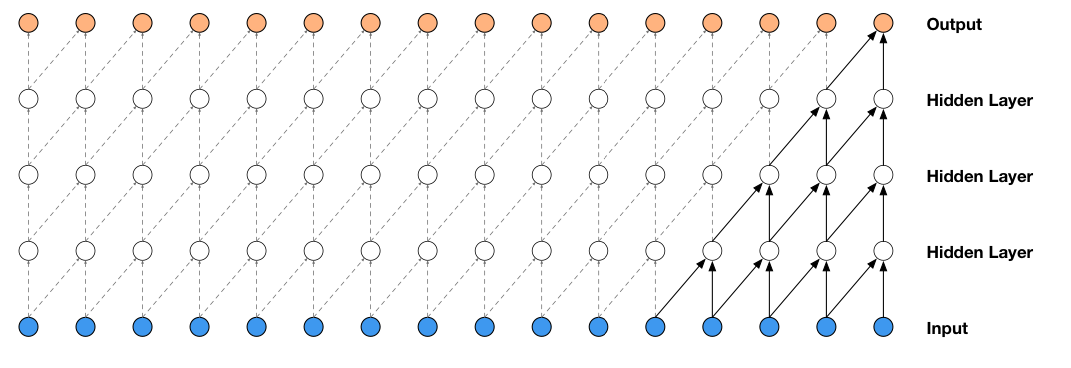
\includegraphics[scale=0.3]{CausalConvolutions.png}
Figure : Visualization of a stack of dilated causal convolutional layers
\linebreak
Source: [@paper_oord_dieleman_2016]

\end{frame}
%%%%%%%%%%%%%%%%%%%%%%%%%%%%%%%%%%%%%%%%%%%%%%%%%%%%%%%%%%%%%%%%%%%%%%%

# Music Production with WaveNet

### Music Production with WaveNet

- "WaveNets can be used to model any audio signal"
\linebreak
- Unlike the TTS experiments networks were not conditioned on an input sequence telling it what to play (such as a musical score)
- Instead : simply let it generate whatever it wanted to
- Fact that directly generating timestep per timestep with deep neural networks works at all for 16kHz audio is really surprising

\vspace{1cm}
Source : [@webpage_oord_dieleman_2016]
\end{frame}
%%%%%%%%%%%%%%%%%%%%%%%%%%%%%%%%%%%%%%%%%%%%%%%%%%%%%%%%%%%%%%%%%%%%%%%

# Implementation Example

### Implementation Example

Let's have a look at the Results Chen written down in \linebreak
following article :

\begin{center}
    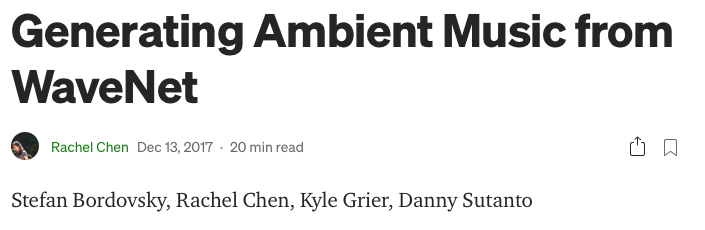
\includegraphics[scale=0.3]{medium.png}
\end{center}

\vspace{1cm}
Source : Medium [@chen_2017]
\end{frame}
%%%%%%%%%%%%%%%%%%%%%%%%%%%%%%%%%%%%%%%%%%%%%%%%%%%%%%%%%%%%%%%%%%%%%%%

## Prerequisites

### Implementation Example - Prerequisites

- Model trained on Tensorflow implementation of WaveNet
- 150 000 steps at a default of 0.001 learning rate
- Amazon Web Services’ p2.xLarge EC2 instance to train the WaveNet model with a GPU
- 118 500 steps trained in approximately 3.5 days ( then AWS costs get to high ) : 
    * with each step taking roughly 2.5 seconds
    * their laptops took approximately 1 minute just to train one step

\vspace{1cm}
Source : Medium [@chen_2017]
\end{frame}
%%%%%%%%%%%%%%%%%%%%%%%%%%%%%%%%%%%%%%%%%%%%%%%%%%%%%%%%%%%%%%%%%%%%%%%

## Results

### Implementation Example - Some Results

- Based on Happy Music from YouTube the model results are : \linebreak
    * \href{https://soundcloud.com/rachachachara/happy-9950-generated?utm_source=clipboard&utm_campaign=wtshare&utm_medium=widget&utm_content=https\%253A\%252F\%252Fsoundcloud.com\%252Frachachachara\%252Fhappy-9950-generated}{\beamergotobutton{9950 steps}} \linebreak
    * \href{https://soundcloud.com/rachachachara/happy-10800-generated?utm_source=clipboard&utm_campaign=wtshare&utm_medium=widget&utm_content=https\%253A\%252F\%252Fsoundcloud.com\%252Frachachachara\%252Fhappy-10800-generated}{\beamergotobutton{10800 steps}}\linebreak
    * \href{https://soundcloud.com/rachachachara/happy-14450-generated?utm_source=clipboard&utm_campaign=wtshare&utm_medium=widget&utm_content=https\%253A\%252F\%252Fsoundcloud.com\%252Frachachachara\%252Fhappy-14450-generated}{\beamergotobutton{14450 steps}}\linebreak
    * \href{https://soundcloud.com/rachachachara/happy-25650-long-generated?utm_source=clipboard&utm_campaign=wtshare&utm_medium=widget&utm_content=https\%253A\%252F\%252Fsoundcloud.com\%252Frachachachara\%252Fhappy-25650-long-generated}{\beamergotobutton{25650 steps}}

\vspace{1cm}
Source : Medium [@chen_2017]
\end{frame}
%%%%%%%%%%%%%%%%%%%%%%%%%%%%%%%%%%%%%%%%%%%%%%%%%%%%%%%%%%%%%%%%%%%%%%%

## Challenges

### Implementation Example - Challenges

- Very much iterations are needed in order to achieve approximately good results
- Model requires at least 20 000 steps to generate something somewhat recognizable
- And around 80 000 steps for something somewhat coherent
- Learning on local machines takes very long for only semi good results

\vspace{1cm}
Source : Medium [@chen_2017]
\end{frame}
%%%%%%%%%%%%%%%%%%%%%%%%%%%%%%%%%%%%%%%%%%%%%%%%%%%%%%%%%%%%%%%%%%%%%%%

## Chances

### Implementation Example - Chances

- Scientist at DeepMind implemented a model playing Piano : 
    * \href{https://storage.googleapis.com/deepmind-media/research/WaveNet/Music/sample_1.wav}{\beamergotobutton{WaveNet Piano example}} [@webpage_oord_dieleman_2016]
- Advantage is, that they input exactly one instrument
- WaveNet achieves good results on simple inputs
- Complex inputs require a lot of learning steps

\end{frame}
%%%%%%%%%%%%%%%%%%%%%%%%%%%%%%%%%%%%%%%%%%%%%%%%%%%%%%%%%%%%%%%%%%%%%%%

# Wrap up

### Wrap up

- WaveNet is basically a good model for generating music
- Good results can be achieved quickly with individual instruments
- If whole songs are used as input, the model has to make significantly more learning steps
- This extensive learning is very computationally, time-consuming and costly

\end{frame}
%%%%%%%%%%%%%%%%%%%%%%%%%%%%%%%%%%%%%%%%%%%%%%%%%%%%%%%%%%%%%%%%%%%%%%%



%%novalidate
\end{markdown}

\begin{frame}
\renewcommand{\bibfont}{\footnotesize}
\frametitle{Bibliography}

\bibliographystyle{apalike}
\bibliography{refs}

\end{frame}


\end{document}
